\documentclass[11pt,a4paper]{article}
\usepackage[T1]{fontenc}
\usepackage[margin=2.3cm]{geometry}
\usepackage{amsmath,amssymb}
\usepackage{graphicx}
\usepackage[dvipsnames]{xcolor}
\usepackage{enumitem}
\usepackage[colorlinks=true,linkcolor=blue,urlcolor=blue]{hyperref}
\setlength{\parskip}{0.6em}
\setlength{\parindent}{0pt}
\begin{document}

\begin{center}{\LARGE\bfseries openbreakeven}\\[0.4em]{\large Find the break-even point of a small business, in three sessions.}\\[0.2em]\small PAN IIT OSS explainer \textbullet{} secondary school to diploma / undergraduate (levels 3-5)\end{center}

\section*{Why this exists}
Every small business pays some costs whether or not it sells anything, and earns a little on each sale. This explainer shows how to find the sales at which income catches up with cost, how safe that point is, and how uncertainty and time change the answer, using only straight lines, a little algebra and a random-number simulation.

\section*{The end goal}
Find the break-even point of a small business. The end goal is to find the break-even point of a small business, and to know how far to trust it. The same ideas appear in pricing, planning a start-up and any decision where a fixed cost must be recovered. All examples are made up and this is general education, not financial advice.

\section*{How the three sessions build up}
\begin{enumerate}[nosep]
\item \textbf{Session 1: Where does income catch up with cost?} (Level 1, conceptual interactive model, 60 min).
\item \textbf{Session 2: The break-even equations: contribution, safety and leverage} (Level 2, mathematical engineering model, 75 min).
\item \textbf{Session 3: Break-even under mix, steps, uncertainty and time} (Level 3, simulation and validation, 90 min).
\end{enumerate}

\section{Session 1: Where does income catch up with cost?}

\subsection*{A. Real-world problem}
You want to run a lemonade stall. Before you sell a single cup you must pay 60 dollars for the stall, a pitcher and a sign. After that each cup costs 50 cents to make and sells for 2 dollars. At the start you are 60 dollars behind. How many cups until your total income has caught up with your total cost? That number is the break-even point. (General education only: the stall is made up and this is not financial advice.)

\subsection*{B. Concept and theory}
The fixed cost F is paid once, however many cups you sell. The variable cost v is paid for every cup. So the total cost after q cups is F + v q, a straight line that starts at F. The income is the price p times q, a straight line that starts at 0. Profit is income minus cost. Each cup earns p - v dollars towards paying off F, so the cups needed are F divided by what one cup earns. If p is not larger than v, a cup earns nothing and income never catches up: there is no break-even.

\begin{itemize}[nosep]
\item F: fixed cost, paid once (dollars)
\item v: variable cost of one cup (dollars per cup)
\item p: price of one cup (dollars per cup)
\item q: cups sold (cups)
\item q*: break-even number of cups (cups)
\end{itemize}

\begin{equation*}
\text{cost}(q)=F+v\,q,\qquad \text{income}(q)=p\,q
\end{equation*}

\begin{equation*}
\text{profit}(q)=p\,q-(F+v\,q)=(p-v)\,q-F
\end{equation*}

\begin{equation*}
q^{*}=\frac{F}{p-v}\quad(\text{only if } p>v)
\end{equation*}

\begin{center}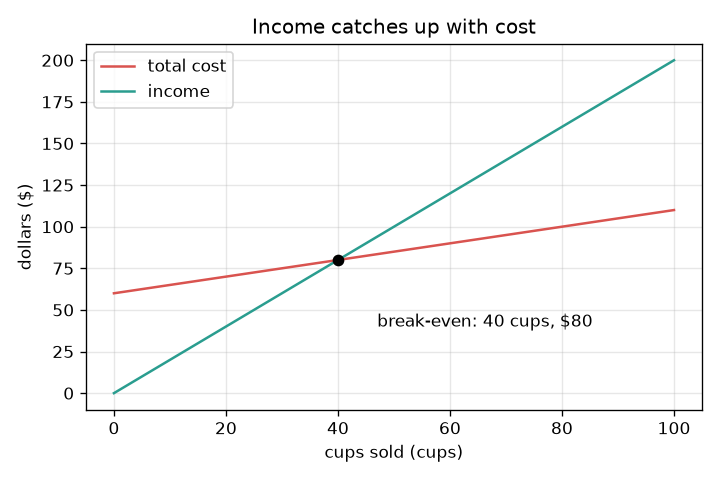
\includegraphics[width=0.85\linewidth]{figures/s01_stall_lines.png}\\\small Cost and income against cups sold: they cross at 40 cups and 80 dollars.\end{center}

\subsection*{E. Worked example}
A stall has fixed cost 60 dollars, sells cups at 2.00 dollars and spends 0.50 dollars per cup. Find the break-even number of cups and check it.
\begin{enumerate}[nosep]
\item Each cup earns 2.00 - 0.50 = 1.50 dollars towards the fixed cost.
\item Cups needed = 60 / 1.50 = 40 cups.
\item Check cost: 60 + 0.50 * 40 = 80 dollars. Check income: 2.00 * 40 = 80 dollars. They are equal.
\item One cup earlier, at 39 cups, the profit is minus 1.50 dollars; one cup later, at 41 cups, it is plus 1.50 dollars.
\end{enumerate}
\textbf{Answer.} Break-even is at 40 cups, where income and cost are both 80 dollars.

\subsection*{F. Questions}
\begin{enumerate}[nosep]
\item \textbf{Conceptual.} A friend says: the stall costs 60 dollars and each cup sells for 2 dollars, so break-even is 60 / 2 = 30 cups. What did they forget?
\item \textbf{Numerical.} A different stall has fixed cost 45 dollars, price 1.50 dollars and a cup cost of 0.60 dollars. Find the break-even cups and check that income equals cost there.
\item \textbf{Graph and simulation interpretation.} On the graph of the first stall, read the cost, the income and the profit at 25 cups. Is the stall ahead or behind?
\item \textbf{Design and optimisation challenge.} Design: the stall will only be open for a short day. Change either the price or the fixed cost so that break-even is at 30 cups or fewer. Which would you pick and what is the risk?
\end{enumerate}

\section{Session 2: The break-even equations: contribution, safety and leverage}

\subsection*{A. Real-world problem}
A made-up neighbourhood bakery sells loaves. Each month it pays 1200 dollars for rent, an oven lease and wages, whether or not anyone buys bread. Each loaf sells for 3.50 dollars and costs 1.40 dollars in flour and energy. The owner expects to sell 800 loaves a month. How many loaves are needed to break even? How far can sales fall before the bakery loses money? How many loaves earn 600 dollars? And how risky is this business compared with another one? (General education only: the bakery and its numbers are made up and this is not financial advice.)

\subsection*{B. Concept and theory}
Profit = income - cost = p q - (F + v q) = (p - v) q - F. The contribution margin p - v is what each loaf contributes towards the fixed cost; its share of the price, (p - v) / p, is the contribution ratio. Setting profit to zero gives the break-even quantity q* = F / (p - v), and the break-even revenue is p q*, which equals F divided by the contribution ratio. The margin of safety, (q - q*) / q, is the share by which sales can fall before the profit disappears. For a target profit T, the quantity is (F + T) / (p - v). The degree of operating leverage, DOL = (p - v) q / profit, tells how strongly profit reacts to sales: a 10 percent change in sales changes profit by DOL times 10 percent. A business with big fixed costs has a high DOL: it gains a lot in good months and loses a lot in bad ones. For the design problem the quantity depends on the price through an estimated demand line, q = a - b p, so profit is a quadratic in p.

\begin{itemize}[nosep]
\item p: price per loaf (dollars per loaf)
\item v: variable cost per loaf (dollars per loaf)
\item F: fixed cost per month (dollars per month)
\item q: loaves sold per month (loaves per month)
\item q*: break-even quantity (loaves per month)
\item T: target profit (dollars per month)
\item a, b: demand line: a = 1675 loaves, b = 250 loaves per dollar (loaves; loaves per dollar)
\item DOL: degree of operating leverage (no unit)
\end{itemize}

\begin{equation*}
\text{profit}=(p-v)\,q-F
\end{equation*}

\begin{equation*}
q^{*}=\frac{F}{p-v},\qquad \text{break-even revenue}=p\,q^{*}=\frac{F}{1-v/p}
\end{equation*}

\begin{equation*}
\text{margin of safety}=\frac{q-q^{*}}{q},\qquad q_T=\frac{F+T}{p-v}
\end{equation*}

\begin{equation*}
\mathrm{DOL}=\frac{(p-v)\,q}{\text{profit}}=\frac{\%\text{ change in profit}}{\%\text{ change in sales}}
\end{equation*}

\begin{equation*}
(p-v)(a-b\,p)-F=T\;\Longrightarrow\; b\,p^{2}-(a+b\,v)\,p+(a\,v+F+T)=0
\end{equation*}

\begin{center}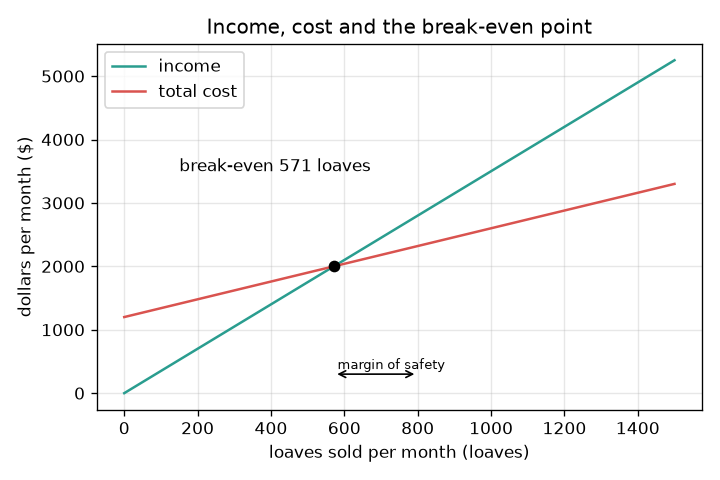
\includegraphics[width=0.85\linewidth]{figures/s02_cvp_lines.png}\\\small Income and cost against loaves: break-even at 571 loaves and the margin of safety up to 800.\end{center}

\subsection*{E. Worked example}
For F = 1200 dollars, p = 3.50, v = 1.40 and 800 loaves a month, find the break-even quantity and revenue, the profit, the margin of safety, the loaves needed for a 600 dollar profit and the DOL. Then test the DOL with a 10 percent change in sales.
\begin{enumerate}[nosep]
\item Contribution margin = 3.50 - 1.40 = 2.10 dollars per loaf; contribution ratio = 2.10 / 3.50 = 0.60.
\item Break-even quantity = 1200 / 2.10 = 571.43 loaves, so 572 whole loaves. Break-even revenue = 1200 / 0.60 = 2000 dollars.
\item Profit at 800 loaves = 2.10 * 800 - 1200 = 480 dollars.
\item Margin of safety = (800 - 571.43) / 800 = 0.2857, about 28.6 percent.
\item Loaves for 600 dollars: (1200 + 600) / 2.10 = 857.14, so 858 whole loaves.
\item DOL = 2.10 * 800 / 480 = 3.5. Test: sales up 10 percent (880 loaves) give profit 648 dollars, which is 35 percent more; sales down 10 percent (720 loaves) give 312 dollars, 35 percent less.
\item Scanning q on a fine grid and stopping when profit reaches zero also finds 571.43, so the formula is right.
\end{enumerate}
\textbf{Answer.} Break-even 571.43 loaves (572 whole) or 2000 dollars; profit 480 dollars at 800 loaves; margin of safety 28.6 percent; 858 loaves for 600 dollars; DOL 3.5, so a 10 percent change in sales moves profit by 35 percent.

\subsection*{F. Questions}
\begin{enumerate}[nosep]
\item \textbf{Conceptual.} Two bakeries both earn 480 dollars at 800 loaves. Bakery X is the one in the worked example. Bakery Y has fixed cost 600 dollars and a variable cost of 2.15 dollars per loaf (more hired help, less rent), both at price 3.50. Which is riskier if sales fall by 10 percent, and why?
\item \textbf{Numerical.} A cafe has F = 900 dollars, price 5 dollars and variable cost 2 dollars. Find the break-even quantity and revenue, and the quantity needed for a 600 dollar profit. Check the units.
\item \textbf{Graph and simulation interpretation.} On the profit-against-loaves line of the worked example, what are the value at 0 loaves, the slope, and the point where it crosses zero? What does each mean?
\item \textbf{Design and optimisation challenge.} Design: with demand q = 1675 - 250 p, variable cost 1.40 dollars and fixed cost 1200 dollars, choose a price that gives 500 dollars profit. How many prices work, what do they sell, and can the bakery reach 600 dollars?
\end{enumerate}

\section{Session 3: Break-even under mix, steps, uncertainty and time}

\subsection*{A. Real-world problem}
The made-up bakery of Session 2 is more complicated than one loaf at one price. It also sells cakes. When it grows it needs a second oven. Its price, its flour cost and its customers are never exactly what the plan says. And the start-up money is paid back slowly, month by month. A single break-even number hides all of that. Can we build a richer model, check it against a formula, and decide which input to watch and which price and oven size to choose? (General education only: made-up numbers, not financial advice.)

\subsection*{B. Concept and theory}
Several products: the sales mix gives each product's share of the units sold; the weighted contribution margin is the mix-weighted average of (p - v), and the break-even units of the whole business are F divided by it. A different mix gives a different break-even, even with the same fixed cost. Step-fixed costs: if one oven bakes at most 700 loaves a month and a second oven adds a fixed cost above that, the fixed cost jumps and so does the profit line, so profit can cross zero several times; we find the crossings by scanning whole loaves and compare them with F\_k / (p - v) for each oven count k. Uncertainty: we draw 20000 random months with a fixed seed from normal distributions for price, variable cost and demand, compute the profit of each and count how many are negative. Reference: if only demand is random, the loss probability is the normal probability that demand is below q*. Sensitivity: change one input by minus and plus 10 percent and note the profit; the input with the widest swing matters most (a tornado chart). Time value: money received later is worth less. Discounting divides month t's cash by (1 + r)\textasciicircum{}t, with monthly rate r = (1 + annual rate)\textasciicircum{}(1/12) - 1. Payback is the first month the running total reaches the start-up cost; NPV is the discounted cash minus the start-up cost. Failure cases: if p \textless{}= v there is no break-even; if demand falls as price rises there are up to two break-even prices, or none if the fixed cost is too big.

\begin{itemize}[nosep]
\item w: weighted contribution margin (dollars per unit)
\item s\_i: share of units for product i (no unit)
\item k: number of ovens (no unit)
\item cap: loaves one oven can bake (700) (loaves per month)
\item sigma: standard deviation of a random input (same as the input)
\item r: monthly discount rate (per month)
\item NPV: net present value (dollars)
\item C0: start-up cost (dollars)
\end{itemize}

\begin{equation*}
w=\sum_i s_i\,(p_i-v_i),\qquad q^{*}_{\text{units}}=\frac{F}{w}
\end{equation*}

\begin{equation*}
F_k=F_1+(k-1)\,\Delta F,\qquad q_k=\frac{F_k}{p-v}\ \text{valid if}\ (k-1)\,\mathrm{cap}<q_k\le k\,\mathrm{cap}
\end{equation*}

\begin{equation*}
\text{profit}=(p-v)\,q-F,\quad p\sim N(\mu_p,\sigma_p^{2}),\ v\sim N(\mu_v,\sigma_v^{2}),\ q\sim N(\mu_q,\sigma_q^{2})
\end{equation*}

\begin{equation*}
P(\text{loss})=\Phi\!\left(\frac{q^{*}-\mu_q}{\sigma_q}\right)\quad(\text{only demand random})
\end{equation*}

\begin{equation*}
r=(1+i)^{1/12}-1,\qquad \mathrm{NPV}=-C_0+\sum_{t=1}^{n}\frac{c_t}{(1+r)^{t}}
\end{equation*}

\begin{equation*}
(p-v)(a-b\,p)=F\;\Longrightarrow\;b\,p^{2}-(a+b\,v)\,p+(a\,v+F)=0\ \ (\text{no real root: no break-even})
\end{equation*}

\begin{center}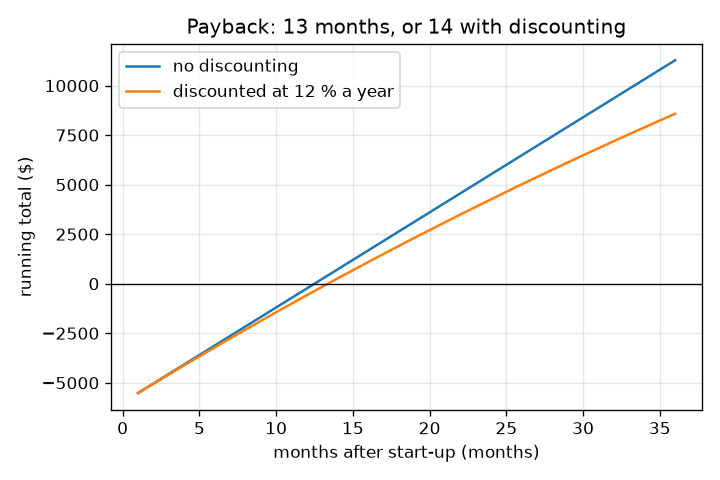
\includegraphics[width=0.85\linewidth]{figures/s03_payback.png}\\\small Running cash total after a 6000 dollar start-up: payback at month 13, month 14 when discounted.\end{center}

\subsection*{E. Worked example}
The bakery sells loaves (price 3.50, variable cost 1.40) and cakes (price 18, variable cost 9) in the unit mix 80 percent loaves and 20 percent cakes, with F = 1200 dollars. Find the break-even, then find the profit crossings if a second oven (900 dollars more) is needed above 700 loaves, and the chance of a loss when only demand is random (mean 800, standard deviation 150, loaves only).
\begin{enumerate}[nosep]
\item Weighted margin = 0.8 * 2.10 + 0.2 * 9.00 = 1.68 + 1.80 = 3.48 dollars per unit.
\item Break-even units = 1200 / 3.48 = 344.8, which is about 275.9 loaves and 69.0 cakes. If the mix shifts to 90 percent loaves the weighted margin is 2.79 and the break-even rises to 430.1 units; at 60 percent loaves it is 246.9 units.
\item Step costs, loaves only: with one oven (fixed 1200) the break-even is 571.43 loaves; profit at 700 loaves is 270 dollars. At 701 loaves the fixed cost is 2100 and the profit is minus 627.90 dollars. With two ovens the break-even is 2100 / 2.10 = 1000 loaves. Scanning whole loaves finds the sign changes at 572 (up), 701 (down) and 1000 (up).
\item Loss chance with only demand random: q* = 571.43, so z = (571.43 - 800) / 150 = -1.524 and P(loss) = 0.0638, about 6.4 percent. The simulation of 20000 months gives about 6.5 percent.
\end{enumerate}
\textbf{Answer.} Break-even 344.8 units for the 80/20 mix (275.9 loaves, 69.0 cakes); with the second oven the profit crosses zero up at 572, down at 701 and up again at 1000 loaves; the loss chance with only demand random is about 6.4 percent by formula and 6.5 percent by simulation.

\subsection*{F. Questions}
\begin{enumerate}[nosep]
\item \textbf{Conceptual.} Why can the break-even of a two-product business go down even though the fixed cost and all prices stay the same?
\item \textbf{Numerical.} A 6000 dollar oven and fit-out earns 480 dollars of cash each month. Find the simple payback month, the discounted payback month at 12 percent a year, and the NPV over 24 months at that rate.
\item \textbf{Graph and simulation interpretation.} In the Monte Carlo histogram, which part of the picture is the loss probability, and what would happen to it if demand became more uncertain (a larger standard deviation) with the same mean?
\item \textbf{Design and optimisation challenge.} Design: the owner may choose the 600, 800 or 1000 loaf oven and a price from 3.00 to 5.00 dollars in 0.25 steps. A choice passes if the loss probability is at most 5 percent, the payback at most 12 months and the margin of safety at least 20 percent. Use \texttt{evaluate} to recommend one choice and explain the trade-off.
\end{enumerate}

\section{Real-world mini-project}
\textbf{Choose the price and the oven size for a made-up bakery.} The owner may buy a 600, 800 or 1000 loaf oven (\texttt{OPTIONS} in the Session 3 lesson gives the monthly fixed cost and the start-up cost of each) and may set any price from 3.00 to 5.00 dollars in steps of 0.25. Demand is 1675 minus 250 times the price (loaves per month) and sales cannot exceed the oven's capacity. Use \texttt{evaluate} from Session 3 to report, for every choice, the break-even quantity, the margin of safety, the loss probability and the payback in months. A choice passes if the loss probability is at most 5 percent, the payback is at most 12 months and the margin of safety is at least 20 percent. Among the passing choices, recommend the one with the highest mean monthly profit. General education only: the numbers are made up.

\section{The path ahead}
\begin{enumerate}[nosep]
\item \textbf{Session 4: Price and demand move together.} A second simulation in which price and demand are negatively correlated (a higher price goes with lower demand).
\item \textbf{Session 5: Shares of the variance.} A function that reports, for price, variable cost and demand, the share of profit variance it explains.
\item \textbf{Session 6: Seasons and a loan.} A 12 month demand pattern with a December peak and a loan repaid in equal monthly instalments.
\item \textbf{Session 7: Design under a risk limit.} A search that adds new oven options and prices, and reports the cheapest design that meets the limit.
\item \textbf{Session 8: A browser lab with live Monte Carlo.} One page with sliders for price, costs, fixed cost and demand, linked to the lines, histogram and tornado chart.
\end{enumerate}

\section{Answers and hints}

\subsection*{Session 1}
\begin{enumerate}[nosep]
\item \textbf{Conceptual.} Hint: Does a cup cost anything to make? Solution: They forgot the variable cost. Each cup brings in 2.00 dollars but also costs 0.50 dollars to make, so it only helps the fixed cost by 1.50 dollars. The right answer is 60 / 1.50 = 40 cups, not 30.
\item \textbf{Numerical.} Hint: Earn per cup = price minus cup cost; then divide. Solution: Each cup earns 1.50 - 0.60 = 0.90 dollars. Cups = 45 / 0.90 = 50. Check: income = 1.50 * 50 = 75 dollars; cost = 45 + 0.60 * 50 = 75 dollars. Equal. Units: dollars divided by dollars per cup gives cups.
\item \textbf{Graph and simulation interpretation.} Hint: Cost line value is 60 plus 0.50 times 25; income is 2.00 times 25. Solution: At 25 cups the cost is 60 + 12.50 = 72.50 dollars and the income is 50 dollars. The profit is 50 - 72.50 = minus 22.50 dollars, a loss: the red line is still above the green line, so the stall is behind.
\item \textbf{Design and optimisation challenge.} Hint: Try price 2.50 with the same fixed cost, and fixed cost 45 with the same price. Then try price 1.00 to see the other direction. Solution: Price 2.50 dollars: each cup earns 2.00, so 60 / 2.00 = 30 cups. Or fixed cost 45 dollars at price 2.00: 45 / 1.50 = 30 cups. Both work. A higher price risks fewer customers (this simple model ignores that); a smaller fixed cost means a cheaper stall, which may be smaller or worse placed. A price of 1.00 dollar would need 60 / 0.50 = 120 cups, so cutting the price a lot pushes break-even far away.
\end{enumerate}

\subsection*{Session 2}
\begin{enumerate}[nosep]
\item \textbf{Conceptual.} Hint: Compute the profit at 720 loaves for each and the percentage drop, or compare the DOL values. Solution: X drops from 480 to 312 dollars, a fall of 35 percent (DOL 3.5). Y has contribution margin 1.35 dollars and profit 1.35 * 720 - 600 = 372 dollars, a fall of 22.5 percent (DOL 2.25). X is riskier because more of its cost is fixed: its profit reacts more strongly to sales. X also gains more in a good month. Operating leverage is risk in both directions.
\item \textbf{Numerical.} Hint: Contribution margin first. Solution: Margin = 5 - 2 = 3 dollars per item. Break-even = 900 / 3 = 300 items and revenue = 300 * 5 = 1500 dollars. For 600 dollars: (900 + 600) / 3 = 500 items. Units: dollars per month divided by dollars per item gives items per month. Sanity check: at 500 items, profit = 3 * 500 - 900 = 600.
\item \textbf{Graph and simulation interpretation.} Hint: The line is (p - v) q - F. Solution: At 0 loaves the profit is minus 1200 dollars: the fixed cost you pay even if you sell nothing. The slope is 2.10 dollars per loaf, the contribution margin. The line crosses zero at 571.43 loaves, the break-even. To the right of it you are in profit.
\item \textbf{Design and optimisation challenge.} Hint: Solve 250 p\textasciicircum{}2 - 2025 p + 4045 = 0, or scan prices on a grid and look for profit = 500. Solution: Two prices work: about 3.58 and 4.52 dollars. At 3.58 the bakery sells about 780 loaves, at 4.52 about 545. Both have margin of safety 500 / 1700 = 29.4 percent, but the cheaper price needs more flour, labour and oven time and has the larger break-even (551 loaves against 384). The most profit is at 4.05 dollars, about 555.6 dollars, so a target of 600 dollars cannot be reached at any price. Trade-off: the higher price gives the same profit with less work but depends on the demand estimate being right.
\end{enumerate}

\subsection*{Session 3}
\begin{enumerate}[nosep]
\item \textbf{Conceptual.} Hint: Think of the weighted contribution margin and the sales mix. Solution: The break-even units are F divided by the weighted margin. If the mix shifts towards the product with the larger margin per unit (cakes, 9.00 dollars, against 2.10 for loaves), the weighted margin rises and the break-even falls: 430.1 units for 90 percent loaves, 344.8 for 80 percent and 246.9 for 60 percent. The fixed cost and prices did not change; only the mix did.
\item \textbf{Numerical.} Hint: Monthly rate = 1.12\textasciicircum{}(1/12) - 1. Add up discounted cash month by month and compare with 6000. Solution: Simple payback: 6000 / 480 = 12.5 months, so the running total first reaches zero in month 13. The monthly rate is 0.9489 percent. Discounted payback is month 14. The 24 month NPV is 4259 dollars (5520 dollars with no discounting). Discounting lowers the value of later cash, so the discounted payback is later and the NPV smaller. Units: dollars and months.
\item \textbf{Graph and simulation interpretation.} Hint: Look at the area left of the zero line, and at how the width changes. Solution: The loss probability is the share of the area (about 9.5 percent of the 20000 months) to the left of zero, the red part. A larger demand standard deviation widens the histogram. The mean profit stays near 480 dollars (the simulated mean is 476) but more months fall below zero, so the loss probability rises.
\item \textbf{Design and optimisation challenge.} Hint: Loop over capacity and price, print loss, payback and mean profit, and filter with \texttt{passes}. Solution: Only the 600 loaf oven at 4.00 and 4.25 dollars passes. The best of them for profit is 4.25 dollars: break-even about 351 loaves, average sales about 546, margin of safety about 36 percent, loss probability about 4 percent, mean profit about 556 dollars a month and payback 9 months. A price of 3.50 fails because the payback is 21 months, and the 1000 loaf oven does not pay back within 36 months at 4.00 dollars because demand is below its capacity most months, so its extra fixed cost is wasted. Trade-off: the biggest oven looks safest for growth but has the highest fixed cost; the small oven loses some sales when demand is high.
\end{enumerate}

\section{How to join}
Read \texttt{CONTRIBUTING.md} in the repository, then pick an issue labelled \texttt{good first issue}. Repository: \url{https://github.com/KrunalPanchal1995/openbreakeven}

\end{document}
